\subsection*{Измерения}


\textbf{Градуировка}. Для начала была произведена градуировка барабана монохроматора УМ-2 по спектру неоновой лампы. Прокрутка барабана допускала приводила к погрешности измерений $\Delta n \sim 15$ у.е. Таким образом былы получены данные таблицы №1 
% \ref{grad_tab}
, где $n$ -- показания на барабане УМ-2 в условных единицах.


Для удобства было построено приближение функции $\lambda(n)$ (рис. \ref{fig:1}). Погрешность в $\lambda$ была оценена, как $\lambda'(n) \Delta n$, что позволило оценить $\chi^2$/ndf. 

\begin{figure}[h]
    \centering
    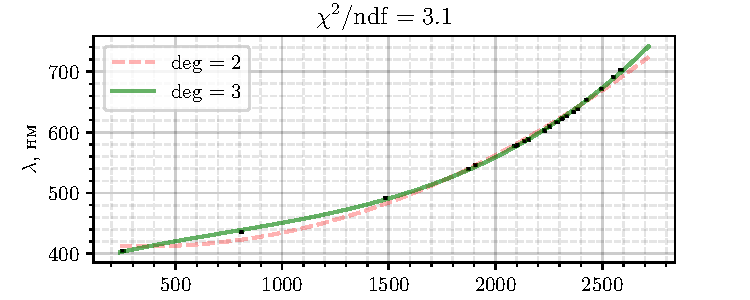
\includegraphics[width=0.7\textwidth]{fig1.pdf}
    \caption{Градуировка монохроматора.}
    \label{fig:1}
\end{figure}

Погрешность полинома в точке $x$ можно оценить, как
\begin{equation*}
    \sigma^2 (x) = (x^3,\, \ldots, x^0) \cdot \,\text{Cov}\,  \cdot (x^3,\, \ldots, x^0)\T,
\end{equation*}
где Cov -- матрица ковариации коэффициентов.


\textbf{Водород}. Найдены и измерены спектральные линии водорода:
\begin{align*}
    \lambda_{\text{H}_{\alpha}}^{m=3}  &= (656 \pm 1) \text{ нм}; \\ 
    \lambda_{\text{H}_{\beta}}^{m=4}   &= (484 \pm 2) \text{ нм}; \\ 
    \lambda_{\text{H}_{\gamma}}^{m=5}  &= (437 \pm 2) \text{ нм}.
\end{align*}
По ним, с учетом формулы \eqref{Balmer}, можем построить линейную зависимость 
$$\frac{1}{\lambda_{m,2}} = R \cdot \left(\frac{1}{4} - \frac{1}{m^2}\right),$$ где коэффициент линейной зависимости будет соответствовать постоянной Ридберга. 

\begin{figure}[h]
    \centering
    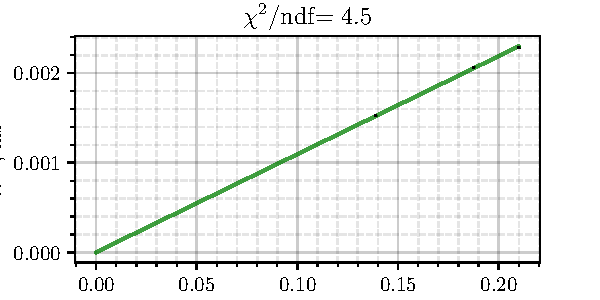
\includegraphics[width=0.6\textwidth]{fig2.pdf}
    \caption{Линеаризация зависимости длины волны перехода от его номера.}
    %\label{fig:}
\end{figure}

Так находим, что
\begin{equation*}
    R = (10.8 \pm 0.3) \text{ мкм},
\end{equation*}
что сходится с табличным значением в рамках погрешности.



\textbf{Йод}.  Для начала найдём длину волны длинноволновой линии, и линии $\nu_{1,0}$, а также $\nu_{1, 6}$ и $\nu_{1,12}$:
\begin{align*}
    \lambda_{1, 0} &= (620 \pm 1) \text{ нм};       
    & E_{1, 0} &= (2.002 \pm 0.002) \text{ эВ};   \\
    \lambda_{1, 6} &= (596 \pm 1) \text{ нм};       
    & E_{1, 6} &= (2.080 \pm 0.003) \text{ эВ};    \\
    \lambda_{\text{гр}} &= (507 \pm 2) \text{ нм};  
    &  E_{\text{гр}} &= (2.447 \pm 0.006) \text{ эВ}, \\
\end{align*}
где $E= h \nu$. Отсюда находим энергию колебательного кванта возбужденного состояния молекулы йоды, по формуле \eqref{iod},
\begin{equation*}
    h \nu_2 = h \frac{\nu_{1, 6} - \nu_{1, 0}}{6} = (0.0130 \pm 0.0007) \text{ эВ}. 
\end{equation*}
Также можем найти $E_2 - E_1 = h \nu_{\text{эл}}$:
\begin{equation*}
    h \nu_{\text{эл}} \approx h \nu_{(1, 0)} - \frac{1}{2} h \nu_2  + \frac{3}{2} h \nu_1 \approx 2 \text{ эВ}.
\end{equation*}
Наконец, находим энергию диссоциации частицы в основном состоянии ($D_1$) и возбужденном состоянии ($D_2$), считая $E_a = 0.94$ эВ:
\begin{align*}
    D_1 &= (1.51 \pm 0.01) \text{ эВ}, \\
    D_2 &= (0.45 \pm 0.01) \text{ эВ}.
\end{align*}








% \begin{table}[h]
%     \centering
%     \caption{Усредненные значения прохождения $\gamma$-лучей}
%     \begin{tabular}{rrrrr}
%     \toprule
%      $n$ &  $N_{\text{Fe}}/s$, с$^{-1}$ &  $N_{\text{Al}}/s$, с$^{-1}$ &  $N_{\text{Pb}}/s$, с$^{-1}$ &  $N_{\text{Cork}}/s$, с$^{-1}$ \\
%     \midrule
%      1 &   4559 &   5581 &   4813 &          \\
%      2 &        &        &   2840 &     7994 \\
%      3 &   1488 &   2414 &   1636 &          \\
%      4 &        &        &    958 &     7729 \\
%      5 &    493 &   1069 &    554 &          \\
%      6 &        &        &    328 &          \\
%      7 &    158 &    472 &    209 &          \\
%      8 &        &    329 &        &     7284 \\
%     \bottomrule
%     \end{tabular}
%     \label{tab:1}
% \end{table}

